
\documentclass[tikz,border=3mm]{standalone}
\begin{document}
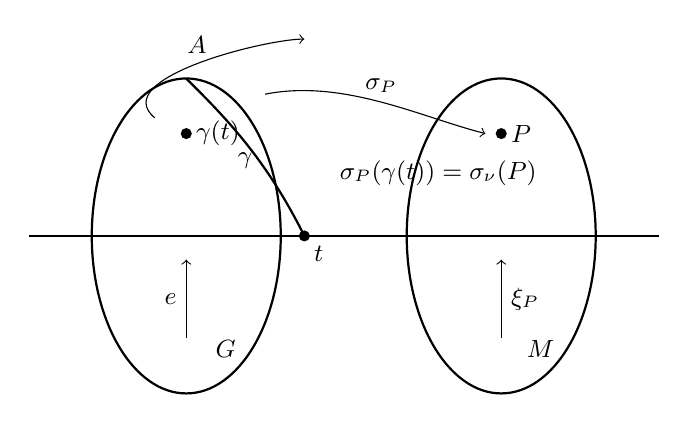
\begin{tikzpicture}[font=\small]

% 坐标轴
% \draw[thick,->] (-0.5,-2.5) -- (-0.5,2.5) node[left] {$\mathbb{R}$};
\draw[thick] (-4,0) -- (4,0);

% 第一组椭圆及内容
\draw[thick] (-2,0) ellipse (1.2cm and 2cm) node[right=0.5cm, below=1.2cm] {$G$};
\draw[->] (-2,-1.3) -- (-2,-0.3) node[midway, left] {$e$};
\draw[thick] (-0.5,0) .. controls (-1,1) and (-1.5,1.5) .. (-2,2) node[pos=0.5, below] {$\gamma$};
\fill (-0.5,0) circle (2pt) node[below right] {$t$};
\fill (-2,1.3) circle (2pt) node[right] {$\gamma(t)$};

% 第二组椭圆及内容
\draw[thick] (2,0) ellipse (1.2cm and 2cm) node[right=0.5cm, below=1.2cm] {$M$};
\fill (2,1.3) circle (2pt) node[right] {$P$};
\draw[->] (2,-1.3) -- (2,-0.3) node[midway, right] {$\xi_P$};

% 椭圆之间的映射关系
\draw[->] (-1,1.8) .. controls (0,2) and (1,1.5) .. (1.8,1.3)
    node[midway, above] {$\sigma_P$};
\draw[->] (-2.4,1.5) .. controls (-3,2) and (-1,2.5) .. (-0.5,2.5) node[midway, above] {$A$};

% 等式标记
\node at (1.2,0.8) {$\sigma_P(\gamma(t)) = \sigma_\nu(P)$};

\end{tikzpicture}
\end{document}
